
%%%%%%%%%%%%%%%%%%%%%%%%%%%%%%%%%%%%%%%%%%%%%%%%%%%%%%%%%%
    \documentclass[twoside,11pt]{article}
    %%%%% PACKAGES %%%%%%
    \usepackage{ctex}
    \usepackage{pgm2016}
    \usepackage{amsmath}
    \usepackage{algorithm}
    \usepackage[noend]{algpseudocode}
    \usepackage{subcaption}
    \usepackage[english]{babel}	
    \usepackage{paralist}	
    \usepackage[lowtilde]{url}
    \usepackage{fixltx2e}
    \usepackage{listings}
    \usepackage{color}
    \usepackage{enumerate}
    \usepackage{booktabs}
    \usepackage{multicol}
    \usepackage{auto-pst-pdf}
    \usepackage{pst-all}
    \usepackage{pstricks-add}
	\usepackage{comment}
	\usepackage{fancybox}
    \usepackage[hidelinks]{hyperref}
    \usepackage{bbding}
    \usepackage{hyperref}
    \usepackage{texnames}
    %%%%% MACROS %%%%%%
    \algrenewcommand\Return{\State \algorithmicreturn{} }
    \algnewcommand{\LineComment}[1]{\State \(\triangleright\) #1}
    \renewcommand{\thesubfigure}{\roman{subfigure}}
    \definecolor{codegreen}{rgb}{0,0.6,0}
    \definecolor{codegray}{rgb}{0.5,0.5,0.5}
    \definecolor{codepurple}{rgb}{0.58,0,0.82}
    \definecolor{backcolour}{rgb}{0.95,0.95,0.92}
    \lstdefinestyle{mystyle}{
       backgroundcolor=\color{backcolour},  
       commentstyle=\color{codegreen},
       keywordstyle=\color{magenta},
       numberstyle=\tiny\color{codegray},
       stringstyle=\color{codepurple},
       basicstyle=\footnotesize,
       breakatwhitespace=false,        
       breaklines=true,                
       captionpos=b,                    
       keepspaces=true,                
       numbers=left,                    
       numbersep=5pt,                  
       showspaces=false,                
       showstringspaces=false,
       showtabs=false,                  
       tabsize=2
    }
    \lstset{style=mystyle}
%%%%%%%%%%%%%%%%%%%%%%%%%%%%%%%%%%%%%%%%%%%%%%%%%%%%%%%%%% 

%%%%%%%%%%%%%%%%%%%%%%%%%%%%%%%%%%%%%%%%%%%%%%%%%%%%%%%%%% 
\newcommand\courseName{Programming in Python}
\newcommand\semester{Fall 2022}
\newcommand\assignmentNumber{1}
\newcommand\studentName{\Large \centering 任课教师: 张涵翠\\王旭刚 2020329621074\\韦杨婧 2020329621199\\池胤杰 2020329621049\\计算机科学与技术全英文授课班20(1)\\}
\newcommand\studentEmail{Email:castamerego@gmail.com}
\newcommand\studentNumber{2020329621074, 2020329621199, 2020329621049}
\newcommand\projectname{Read-Book ``智能知识侦查助手''}
\newcommand\studentClass{\centering}
%%%%%%%%%%%%%%%%%%%%%%%%%%%%%%%%%%%%%%%%%%%%%%%%%%%%%%%%%%
\renewcommand{\thefootnote}{\fnsymbol{footnote}}
\newenvironment{boxedlaw}[1]
{\begin{Sbox}\begin{minipage}{#1}\setcounter{mpfootnote}{\value{footnote}}}
		{\end{minipage}\end{Sbox}\begin{center}\shadowbox{\TheSbox}
		\setcounter{footnote}{\value{mpfootnote}}\end{center}}

\renewcommand*\thempfootnote{\fnsymbol{mpfootnote}}



\ShortHeadings{Coursework of ZSTU - \courseName}{\projectname}
    
\begin{document}

\begin{figure}[H]
    \centering
    
\includegraphics[width=1\columnwidth]{figures/zstu-logo.png}
\end{figure}

\title{\Huge Python 程序设计\\ \vspace{1.5cm} Read-Book ``智能知识侦查助手''(9) \\ \vspace{1.5cm} \huge 2022-2023-1 \\ \vspace{0.8cm}}

\author{\name \studentName{}
    \addr
}

\maketitle
\thispagestyle{empty}
\newpage



\phantomsection\addcontentsline{toc}{section}{Author}\tolerance=500

\begin{center}
    王旭刚\textsuperscript{1*},
    韦杨婧\textsuperscript{2},
    池胤杰\textsuperscript{3}
    \\
    \bigskip
    \textbf{1*} Leader, back-end and webcrawer design and implementation
    \\
    \textbf{2} Team member, front-end design and implementation
    \\
    \textbf{3} Team member, question data collect, data cleaning
    \\
    \bigskip
    %
\end{center}



\phantomsection\addcontentsline{toc}{section}{Abstruct}\tolerance=500

\begin{center}
    \Large\textbf{Abstruct}
\end{center}

% 第一段为研究背景、意义或目的,第二段为本文的结构

Our team's course design is called ``Read-Book'', an Intelligent Knowledge Scouting Assistant. Our work can be roughly devided to these parts:  1. We used webcrawer to gather data of the top 200 rated books from book.douban.com. and store data into database. 2. Based on those 200 books, we developed different ways to collect and generate question about them. 3. Derive templates to pick questions to form questionnaire. 4. Create GUI interface through Web-App. 5. Analysis, assess and evaluate user statistics from multi angles. 6. Implement an Intuitive Data Visualization for user.

We used \emph{Python} as the main programming language. Use \emph{flask} library to manipulate html, css, javascript for front-end; \emph{requests, BeautifulSoup4} library for webcrawing data; and \emph{pymysql} library for back-end programming. For more information, you can click  \href{https://github.com/Casta-mere/Read-Book}{\textbf{\emph{here}}} to view our Github Repository and click \href{http://47.116.46.195/}{\textbf{\emph{here}}} to view our product page. \\ \vspace{1.0cm}

Key words: Python, Webcrawer, Question/Questionnaire Generating, Object-Orinted Programming\cite{wikiforoop}, Web--App


\pagenumbering{Roman}
\newpage

\phantomsection\addcontentsline{toc}{section}{课题执行(文档修订)记录表}\tolerance=500

\begin{center}
    \Large\textbf{课题执行(文档修订)记录表}
\end{center}

\begin{table}[H]
    \centering
    \caption{课题执行(文档修订)记录表(按姓氏拼音顺序排列)}
    \setlength{\tabcolsep}{4mm}{
        \begin{tabular}{|c|c|c|c|c|}
            \hline
            日期       & 版本 & 修订内容             & 执行人                 & 修订人 \\
            \hline
            2022.11.06 & 1.0  & 分析需求             & 池胤杰、王旭刚、韦杨婧 & 王旭刚 \\
            \hline
            2022.11.07 & 1.1  & 系统框架设计         & 池胤杰、王旭刚、韦杨婧 & 王旭刚 \\
            \hline
            2022.11.08 & 1.2  & 用户、书籍数据库设计 & 王旭刚、韦杨婧         & 韦杨婧 \\
            \hline
            2022.11.09 & 1.9  & 总结、问题添加       & 王旭刚                 & 王旭刚 \\
            \hline
            2022.11.16 & 2.1  & 修改README           & 王旭刚                 & 韦杨婧 \\
            \hline
            2022.11.17 & 2.2  & 完善摘要             & 王旭刚                 & 王旭刚 \\
            \hline
            2022.11.17 & 2.3  & 问题数据增加至前29本 & 池胤杰                 & 王旭刚 \\
            \hline
            2022.11.18 & 3.1  & 成功在服务器部署     & 王旭刚                 & 韦杨婧 \\
            \hline
            2022.11.19 & 3.2  & 问题数据增加至200本  & 池胤杰                 & 王旭刚 \\
            \hline
            2022.11.20 & 3.3  & 实现了数据展示界面   & 韦杨婧                 & 韦杨婧 \\
            \hline
            2022.11.20 & 3.4  & 实现了批改试卷       & 王旭刚                 & 王旭刚 \\
            \hline
            2022.11.21 & 3.5  & 总结、问题添加       & 王旭刚                 & 王旭刚 \\
            \hline
        \end{tabular}}

    \label{tab:tab1}
\end{table}

\newpage



\begin{center}
    \tableofcontents
\end{center}
\thispagestyle{empty}
\newpage



\pagenumbering{arabic}


\section{系统设计}
\subsection{概要设计}
\subsubsection{系统框架设计}

本项目为一个基于python的web应用,主要由前端和后端组成,前端主要负责用户界面的展示,后端主要负责数据的处理和存储。前端使用使用flask框架,同时使用html、css、javascript,后端使用python语言,数据库使用mysql。

在书籍数据,问题数据获取方面,使用了python的requests、selenium库,通过爬虫的方式获取数据,再使用BeautifulSoup4、re等库进行数据处理与清洗,最后后使用python的pymysql库将数据存储到mysql数据库中。

在后端的全部设计中,我们在动手前先进行了讨论,确定了我们的系统的架构,以及各个模块的功能,最后确定了我们的系统的框架图,如图\ref{fig:fig1}所示,整体体现了面向对象的设计思想。

\begin{figure}[H]
    \centering
    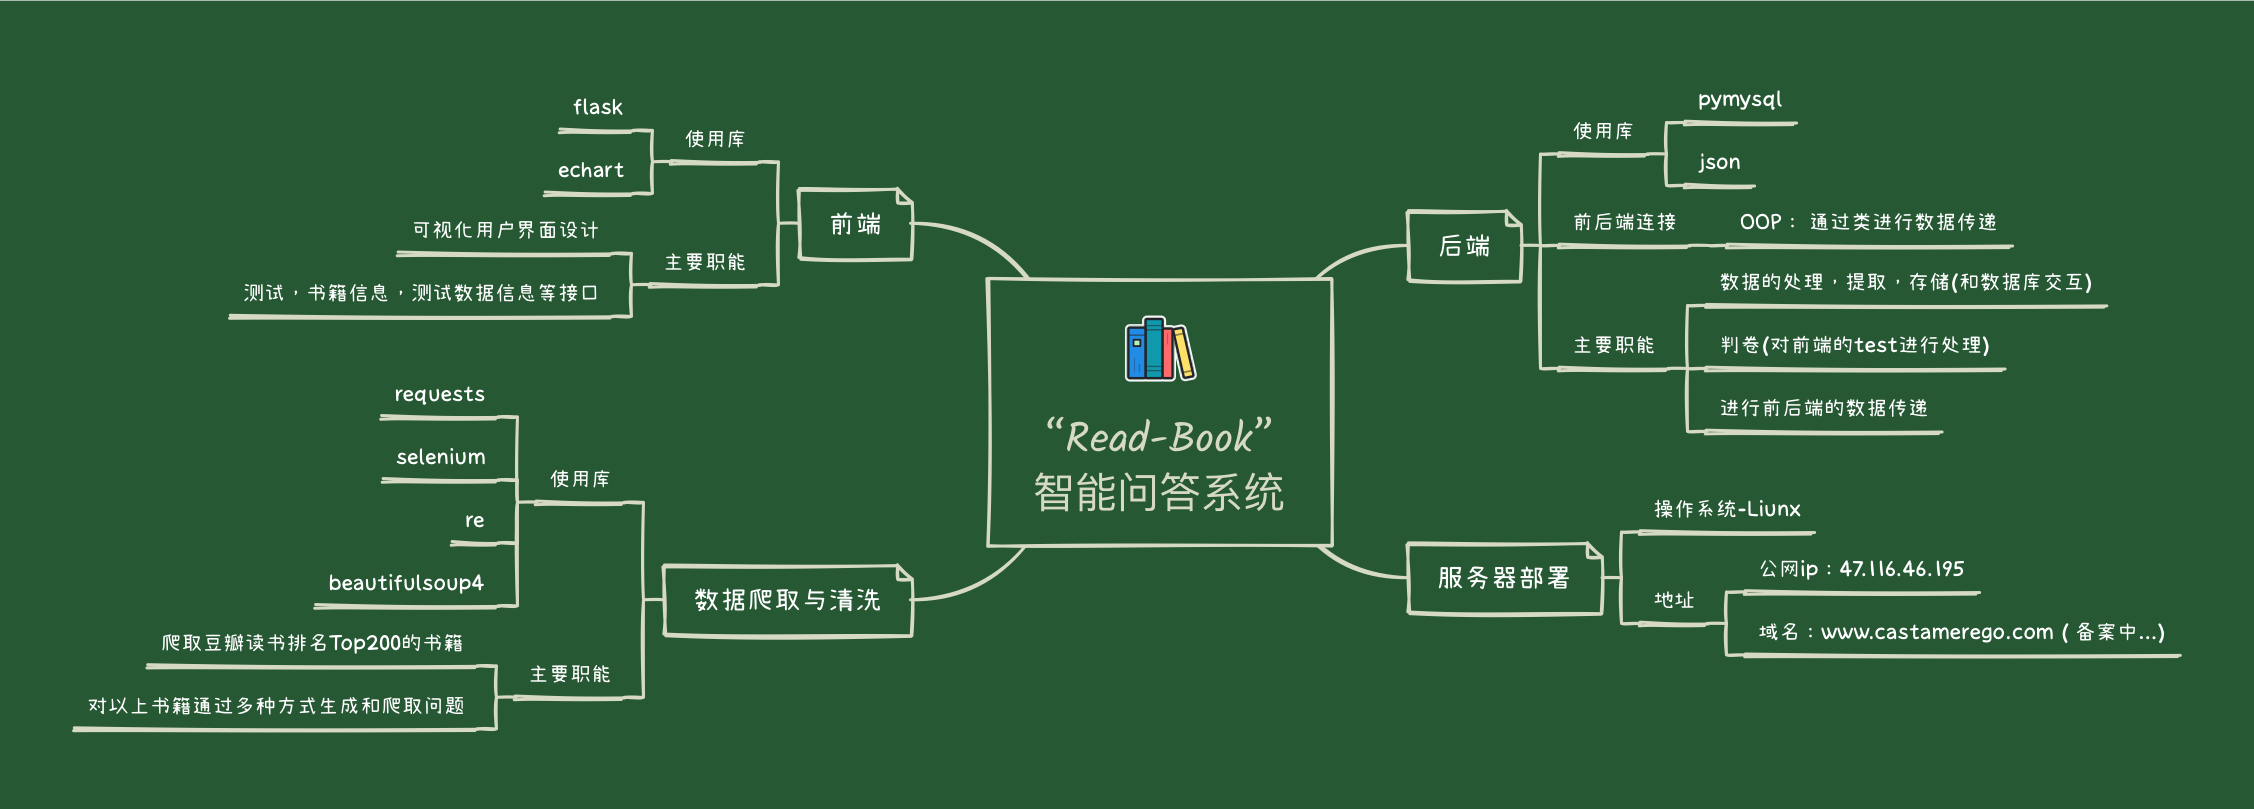
\includegraphics[width=1\columnwidth]{figures/系统框架设计.jpg}
    \caption{系统框架设计}
    \label{fig:fig1}
\end{figure}
\subsubsection{系统功能设计}

经过需求分析和头脑风暴过后,我们共同确定了我们的系统的功能:
\begin{itemize}
    \item 书籍/问题数据的获取
    \item 用户注册/登录/登出
    \item 全部书籍信息概览
    \item 书籍信息测试(按照多种方式:按照书籍、按照题目类型、全部题库随机抽样等)
    \item 测试结果分析以及可视化展示
\end{itemize}

\subsection{功能设计}

\subsubsection{功能1 -- 书籍/问题数据的获取}
该部分主要是通过爬虫的方式获取数据,然后进行数据清洗,最后将数据存储到数据库中。首先是爬取豆瓣的Top200书籍信息,再根据爬出的书籍通过多种方式获取书籍的问题数据,最后将数据存储到数据库中。

获取问题时,有以下几种方式:
\begin{itemize}
    \item 通过数据库中的书籍信息,生成概念类问题,如:《三体》的作者是谁?
    \item 通过手动信息搜集,如搜集百度文库,豆瓣评论等
\end{itemize}

\vspace{0.5cm}

\subsubsection{功能2 -- 用户注册/登录/登出}
该部分主要是实现用户的注册、登录、登出功能。主要需要实现的功能有:
\begin{itemize}
    \item 用户注册 -- 用户输入用户名、密码、邮箱等信息,注册成功后,将用户信息存储到数据库中
    \item 用户登录 -- 用户输入用户名、密码,登录成功后,将用户信息存储到当前对话中
    \item 用户登出 -- 用户登出后,将用户信息从当前对话中删除
\end{itemize}

\vspace{0.5cm}

\subsubsection{功能3 -- 全部书籍信息概览}
该部分主要实现对书籍信息的概览,主要包括全部(200本)书籍的信息概览,以及每本书的详细信息显示,在书籍的详细信息显示界面将加入针对单本书籍的信息测试,详见功能4。


\vspace{0.5cm}

\subsubsection{功能4 -- 书籍信息测试}
该部分主要实现对书籍信息的测试,使用在功能1中爬取的书籍信息,通过多种方式进行测试,包括:
\begin{itemize}
    \item 按照书籍进行测试 -- 用户选择一本书,然后进行测试
    \item 按照题目类型进行测试 -- 用户选择一种题目类型,然后进行测试
    \item 全部题库随机抽样 -- 用户选择随机抽样,然后进行测试
\end{itemize}

\vspace{0.5cm}

\subsubsection{功能5 -- 测试结果分析以及可视化展示}
该部分主要实现对测试结果的分析以及可视化展示,主要包括:
\begin{itemize}
    \item 测试结果分析 -- 对测试结果进行分析,包括正确率、错误率、各种类别题目的正确、错误条数、答题时长。以及对单次和多次的测试结果梳理
    \item 测试结果可视化展示 -- 对测试结果进行可视化展示,包括雷达图,柱状图,分析文本等
\end{itemize}
\subsection{数据库设计}

在本项目中,所有数据库均使用sqlserver数据库,以Python的\emph{pymysql}库进行操作,共有四个表,分别为书籍、用户、题目、测试结果表。
\subsubsection{数据表1 -- 书籍}

书籍数据库主要用于豆瓣爬取出的200本书籍的信息,包括书名、作者、出版社、出版时间、评分、评价人数、标签、简介、题目等信息。种类可大致分为中国与外国书籍,其在部分条目中有些许差异,具体如表\ref{tab:tabforbook}所示。我们将其在豆瓣中的排名作为书籍的id,以便于后续的操作。
\begin{table}[H]
    \centering
    \caption{书籍储数据存---数据库设计}
    \begin{tabular}{|l|l|c|c|c|}
        \hline
        Attribute     & Translation & Type    & Chinese Book & Foreign Book \\
        \hline
        Id            & 排名        & int     & \Checkmark   & \Checkmark   \\
        \hline
        Name          & 书名        & varchar & \Checkmark   & \Checkmark   \\
        \hline
        Author        & 作者        & varchar & \Checkmark   & \Checkmark   \\
        \hline
        Country       & 国家        & varchar & \Checkmark   & \Checkmark   \\
        \hline
        Publisher     & 出版社      & varchar & \Checkmark   & \Checkmark   \\
        \hline
        Year          & 出版日期    & varchar & \Checkmark   & \Checkmark   \\
        \hline
        Page          & 页数        & varchar & \Checkmark   & \Checkmark   \\
        \hline
        Price         & 定价        & varchar & \Checkmark   & \Checkmark   \\
        \hline
        Frame         & 装帧        & varchar & \Checkmark   & \Checkmark   \\
        \hline
        Category      & 丛书        & varchar & \Checkmark   & \Checkmark   \\
        \hline
        Isbn          & isbn码      & varchar & \Checkmark   & \Checkmark   \\
        \hline
        Star          & 评分        & float   & \Checkmark   & \Checkmark   \\
        \hline
        Comment num   & 评价数量    & int     & \Checkmark   & \Checkmark   \\
        \hline
        Brief         & 简介        & varchar & \Checkmark   & \Checkmark   \\
        \hline
        Douban bookid & 豆瓣id      & varchar & \Checkmark   & \Checkmark   \\
        \hline
        Link          & 链接        & varchar & \Checkmark   & \Checkmark   \\
        \hline
        Name o        & 原作名      & varchar & \XSolidBrush & \Checkmark   \\
        \hline
        Trans         & 译者        & varchar & \XSolidBrush & \Checkmark   \\
        \hline
    \end{tabular}

    \label{tab:tabforbook}
\end{table}

\subsubsection{数据表2 -- 用户}
用户数据库主要用于用户的注册、登录、登出等操作,包括用户名、密码、电话、性别、个人简介等信息。具体如表\ref{tab:tabforuser}所示。
\begin{table}[H]
    \centering
    \caption{用户数据储存---数据库设计}
    \setlength{\tabcolsep}{11mm}{
        \begin{tabular}{|c|c|c|}
            \hline
            Attribute & Type    & Translation \\

            \hline
            Id        & int     & 编号        \\
            \hline
            Name      & varchar & 姓名        \\
            \hline
            Gender    & char    & 性别        \\
            \hline
            Telephone & varchar & 电话        \\
            \hline
            Password  & varchar & 密码        \\
            \hline
            Brief     & varchar & 简介        \\
            \hline
        \end{tabular}
    }
    \label{tab:tabforuser}
\end{table}

\subsubsection{数据表3 -- 题目}
题目数据库主要用于题目的储存,包括题目、选项、答案、问题类别、书籍id、内容类别等信息。具体如表\ref{tab:tabforquestion}所示。其中选项至多为4项,问题的种类有单选题和判断题,内容类别有书籍简介、主要人物、作者、情节等,具体如表\ref{tab:tabforquestioncate}所示。
\begin{table}[H]
    \centering
    \caption{问题储存---数据库设计}
    \setlength{\tabcolsep}{7mm}{
        \begin{tabular}{|c|c|c|c|}
            \hline
            Attribute    & Type    & Translation    & Note                       \\
            \hline
            Id           & int     & 关联书本的id   &                            \\
            \hline
            Question     & varchar & 问题           &                            \\
            \hline
            Type         & int     & 类别           & 0-判断, 1-单选             \\
            \hline
            Question num & int     & 选项数量       &                            \\
            \hline
            C1           & varchar & 选项1          &                            \\
            \hline
            C2           & varchar & 选项2          &                            \\
            \hline
            C3           & varchar & 选项3          &                            \\
            \hline
            C4           & varchar & 选项4          &                            \\
            \hline
            Ans          & varchar & 正确选项       & 必须与某个选项完全相同     \\
            \hline
            Category     & varchar & 问题内容的类别 & 如: 问作者, 书中人物, 情节 \\
            \hline
        \end{tabular}
    }
    \label{tab:tabforquestion}
\end{table}

\begin{table}[H]
    \centering
    \caption{问题内容类别}
    \setlength{\tabcolsep}{13mm}{
        \begin{tabular}{|c|c|}
            \hline
            Type     & Translation \\
            \hline
            figure   & 人物        \\
            \hline
            writer   & 作者        \\
            \hline
            main     & 主旨        \\
            \hline
            content  & 情节        \\
            \hline
            detail   & 细节        \\
            \hline
            anecdote & 其他        \\
            \hline
        \end{tabular}
    }
    \label{tab:tabforquestioncate}
\end{table}

\subsubsection{数据表4 -- 测试结果}
测试结果数据库主要用于测试结果的储存,包括用户id、书籍id、测试结果、测试时间等信息。具体如表\ref{tab:tabfortest}所示。
\begin{table}[H]
    \centering
    \caption{测试数据储存---数据库设计}
    \setlength{\tabcolsep}{7mm}{
        \begin{tabular}{|c|c|c|}
            \hline
            Attriubute  & Type  & Translation              \\
            \hline
            Userid      & int   & 用户id                   \\
            \hline
            Score       & float & 得分                     \\
            \hline
            Start       & int   & 开始时间(使用unix时间戳) \\
            \hline
            End         & int   & 结束时间(使用unix时间戳) \\
            \hline
            Duration    & int   & 答题时长(秒)             \\
            \hline
            A1          & int   & 人物形象相关答对个数     \\
            \hline
            A2          & int   & 作者相关答对个数         \\
            \hline
            A3          & int   & 主题相关答对个数         \\
            \hline
            A4          & int   & 情节相关答对个数         \\
            \hline
            A5          & int   & 细节相关答对个数         \\
            \hline
            B1          & int   & 人物形象相关题目总数     \\
            \hline
            B2          & int   & 作者相关题目总数         \\
            \hline
            B3          & int   & 主题相关题目总数         \\
            \hline
            B4          & int   & 情节相关题目总数         \\
            \hline
            B5          & int   & 细节相关题目总数         \\
            \hline
            questionnum & int   & 问题数量                 \\
            \hline
            rightnum    & int   & 正确数量                 \\
            \hline
            wrongnum    & int   & 错误数量                 \\
            \hline
            emptynum    & int   & 未回答数量               \\
            \hline
        \end{tabular}
    }
    \label{tab:tabfortest}
\end{table}

\section{系统实现}
\subsection{前端实现}
\subsubsection{页面 1 -- Log/Register}
\subsubsection{页面 2 -- Home}
\subsubsection{页面 3 -- Book}
\subsubsection{页面 4 -- Test}
\subsubsection{页面 5 -- Statistics}
\subsubsection{页面 6 -- Profile}

\newpage
\subsection{后端实现 -- UML类图}
\begin{figure}[htbp]
    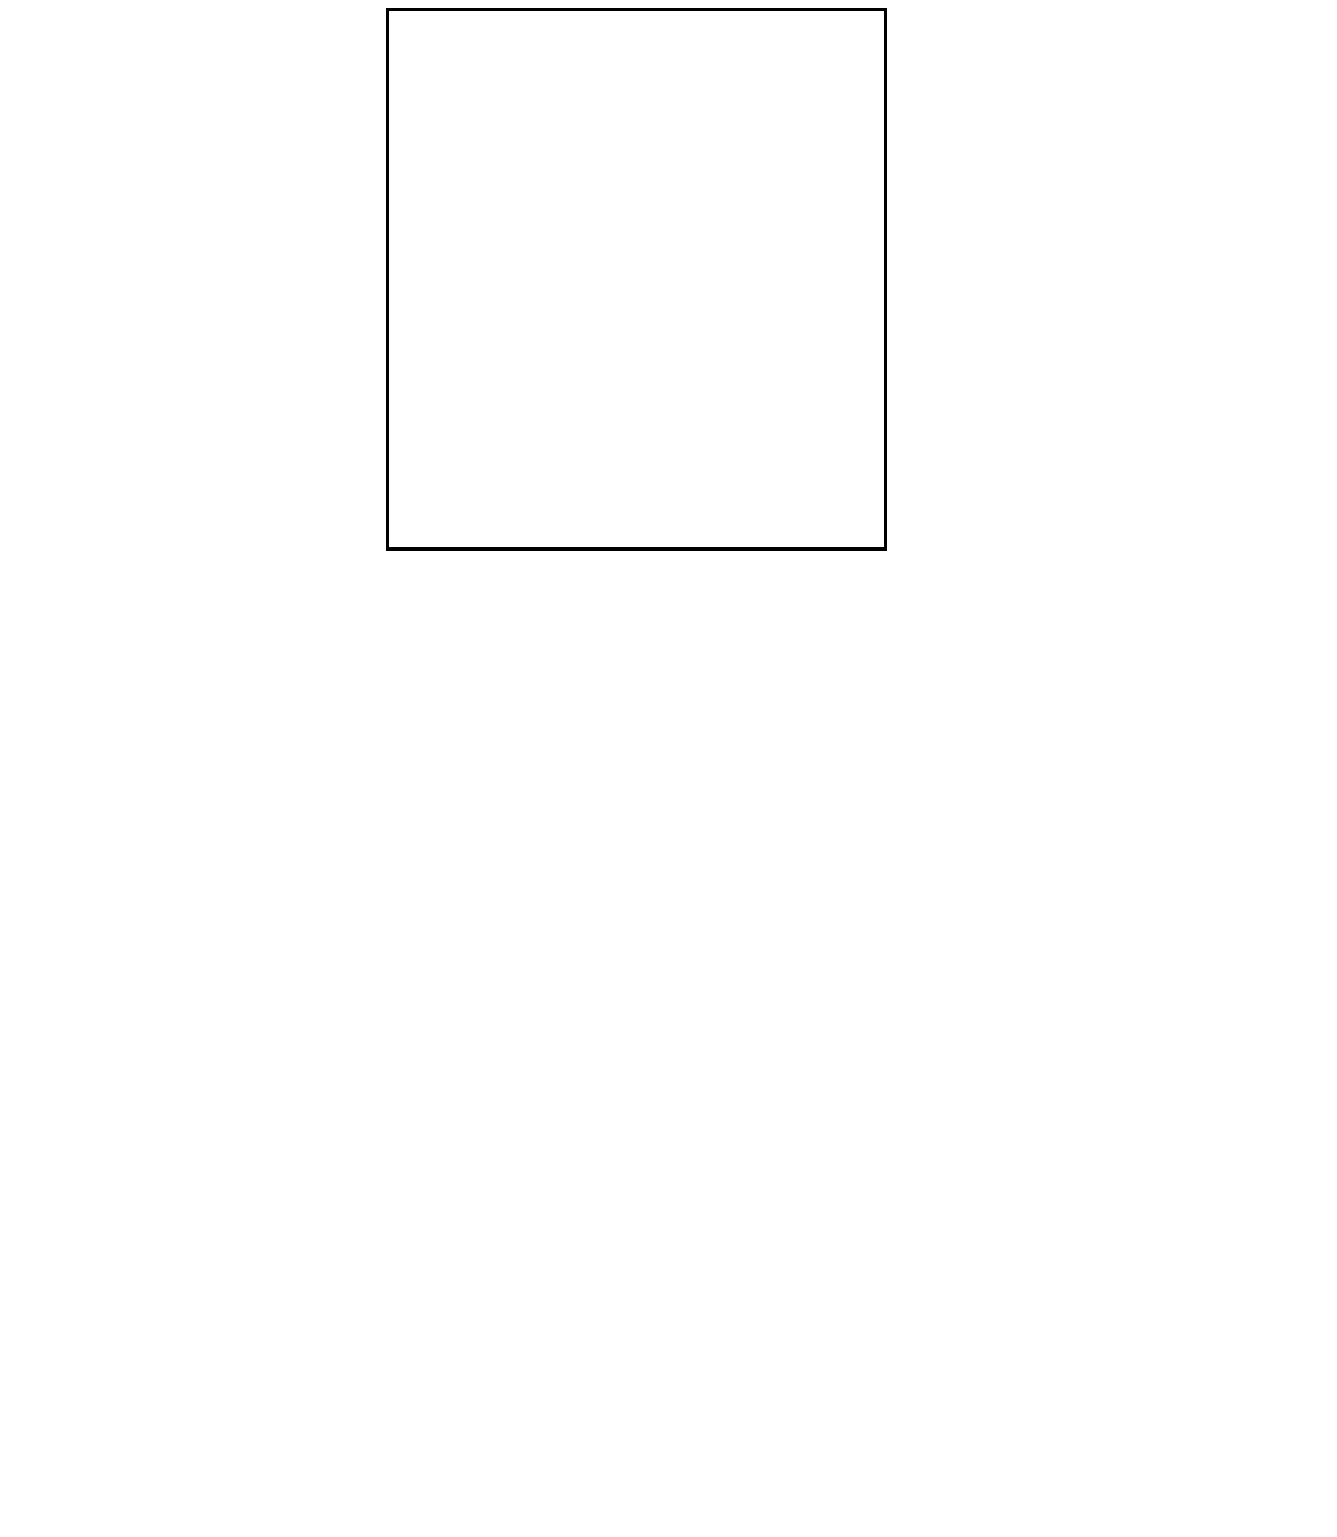
\includegraphics[width=1\columnwidth]{figures/backenduml.pdf}
    \caption{后端UML图}
    \label{fig:backenduml}
\end{figure}
\subsection{前后端交互}

\subsubsection{用户注册/登录/登出}

\begin{figure}[H]
    \centering
    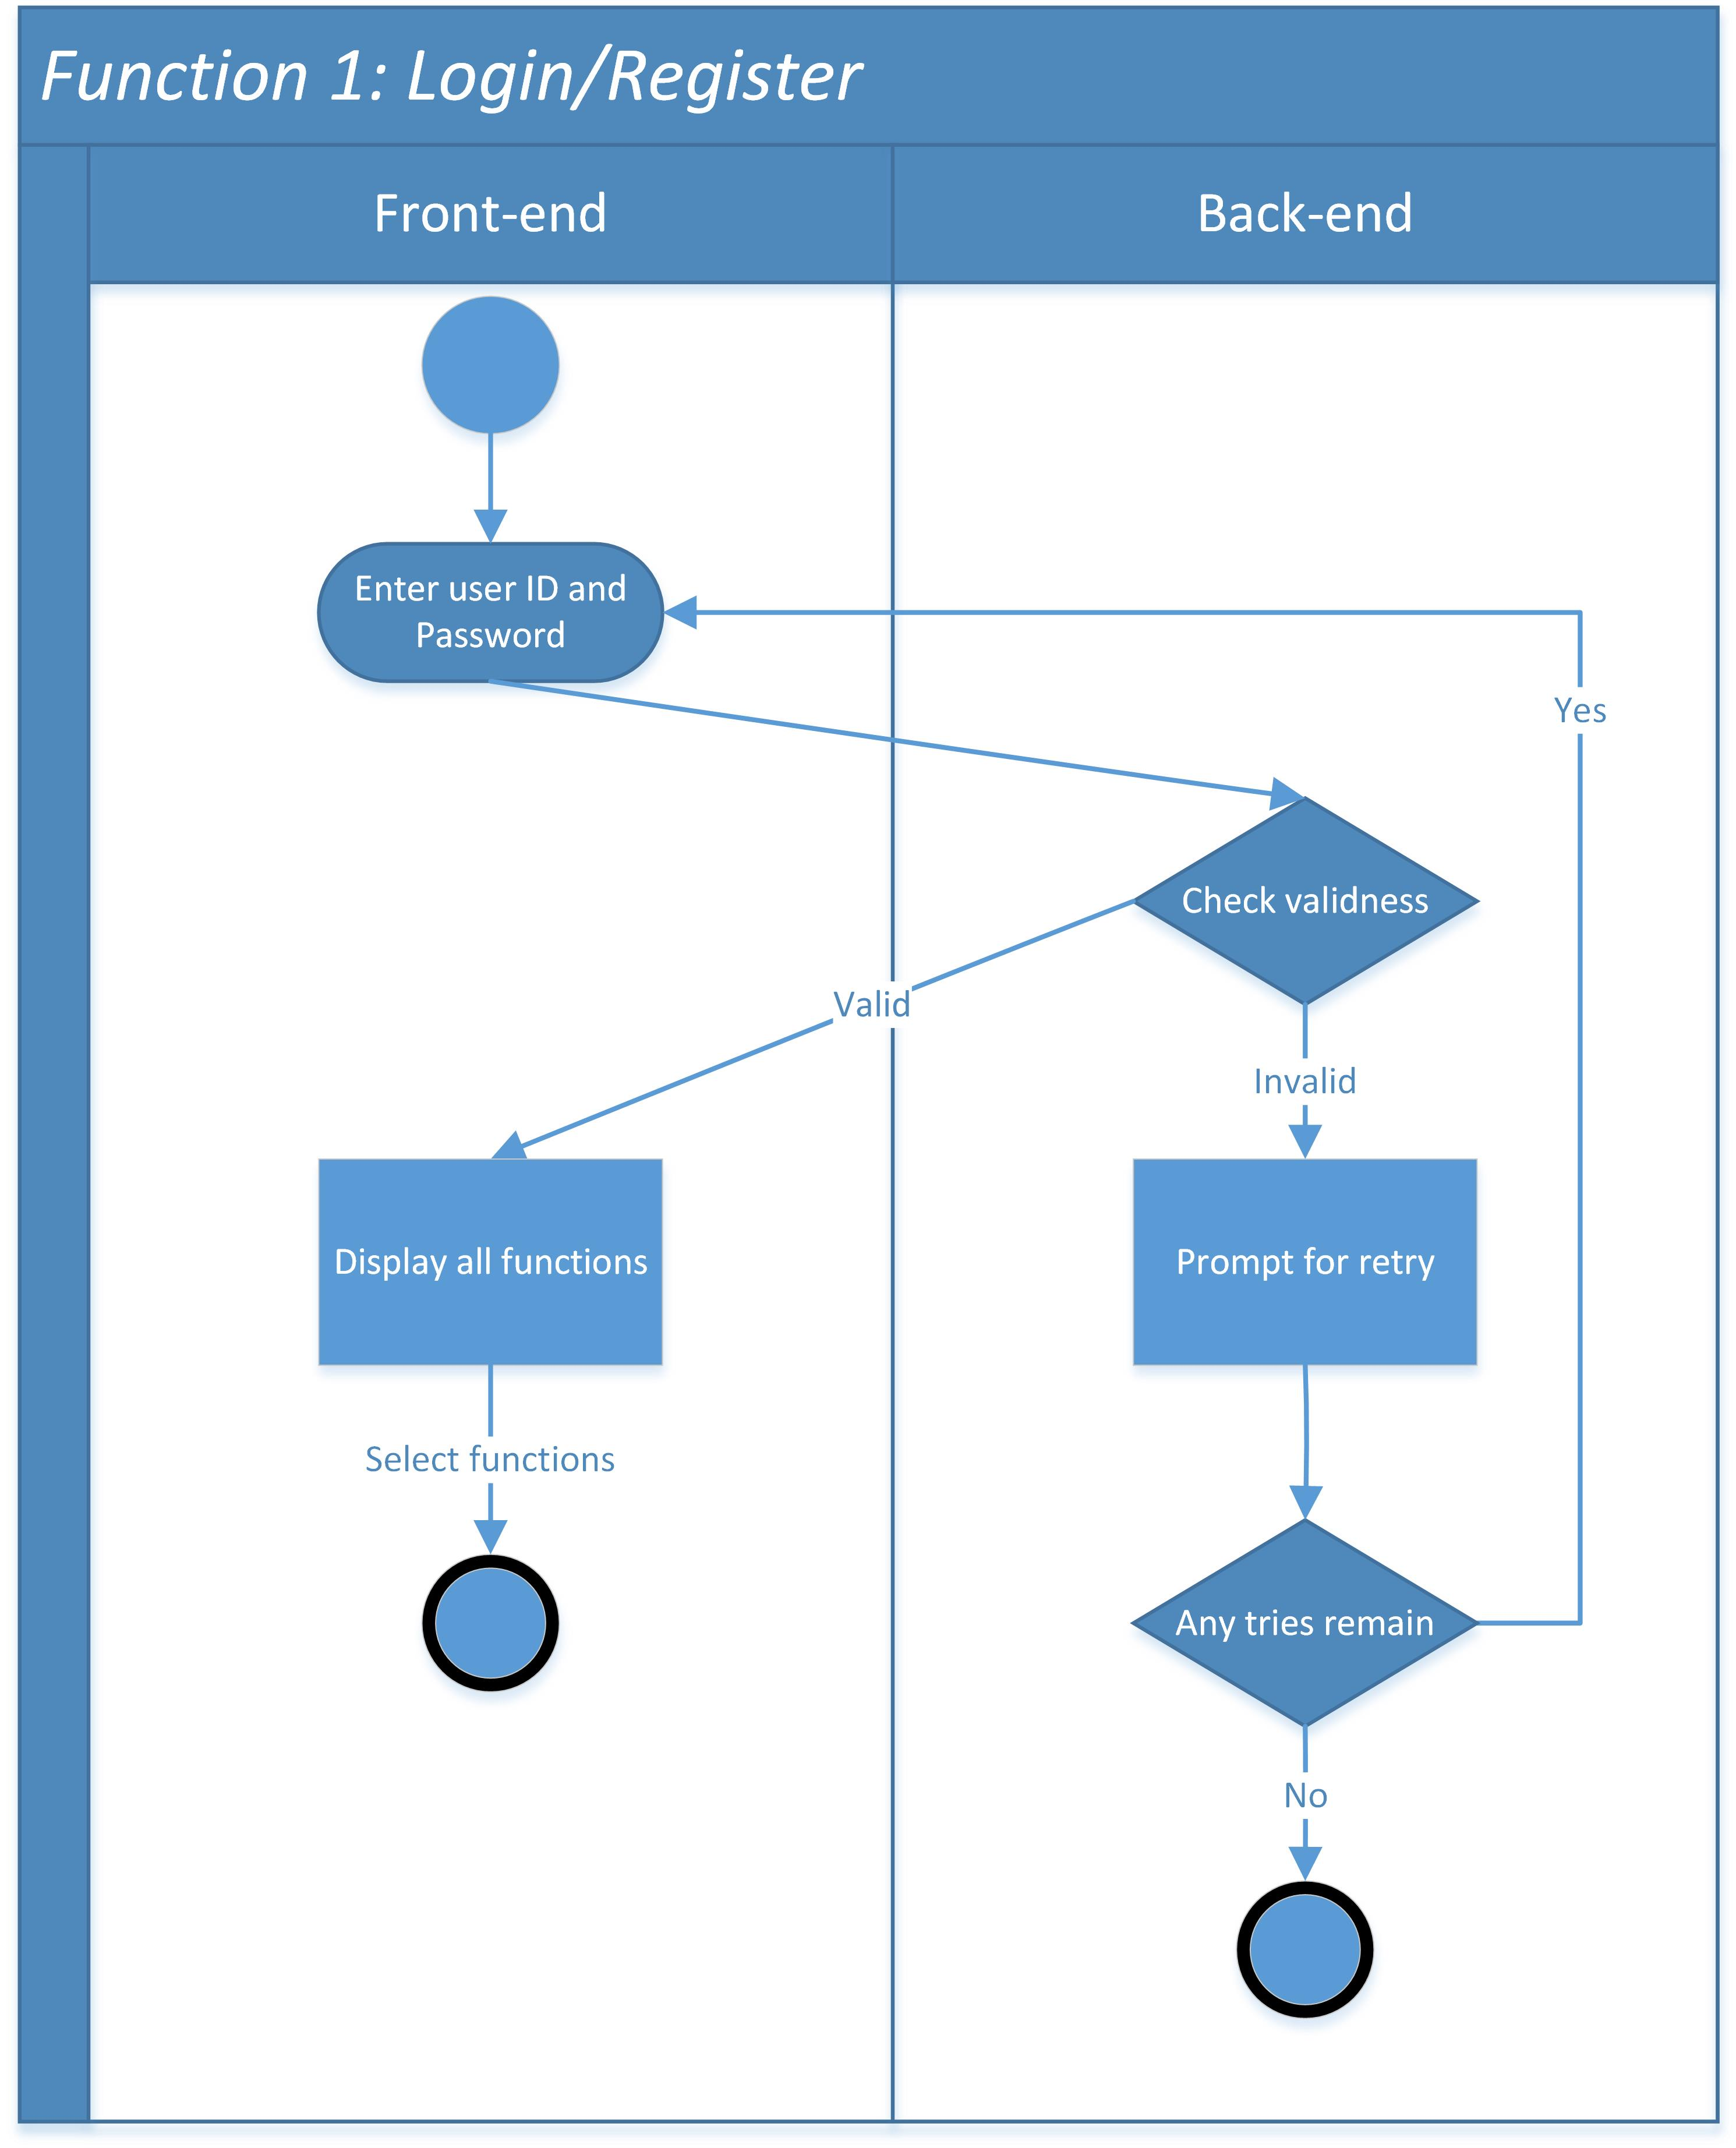
\includegraphics[width=0.9\columnwidth]{SwimLaneDiagram/Usecase_1.jpg}
    \caption{前后端交互:用户注册/登录/登出}
    \label{fig:userlogin}
\end{figure}
\newpage
\subsubsection{全部书籍信息预览}
\begin{figure}[H]
    \centering
    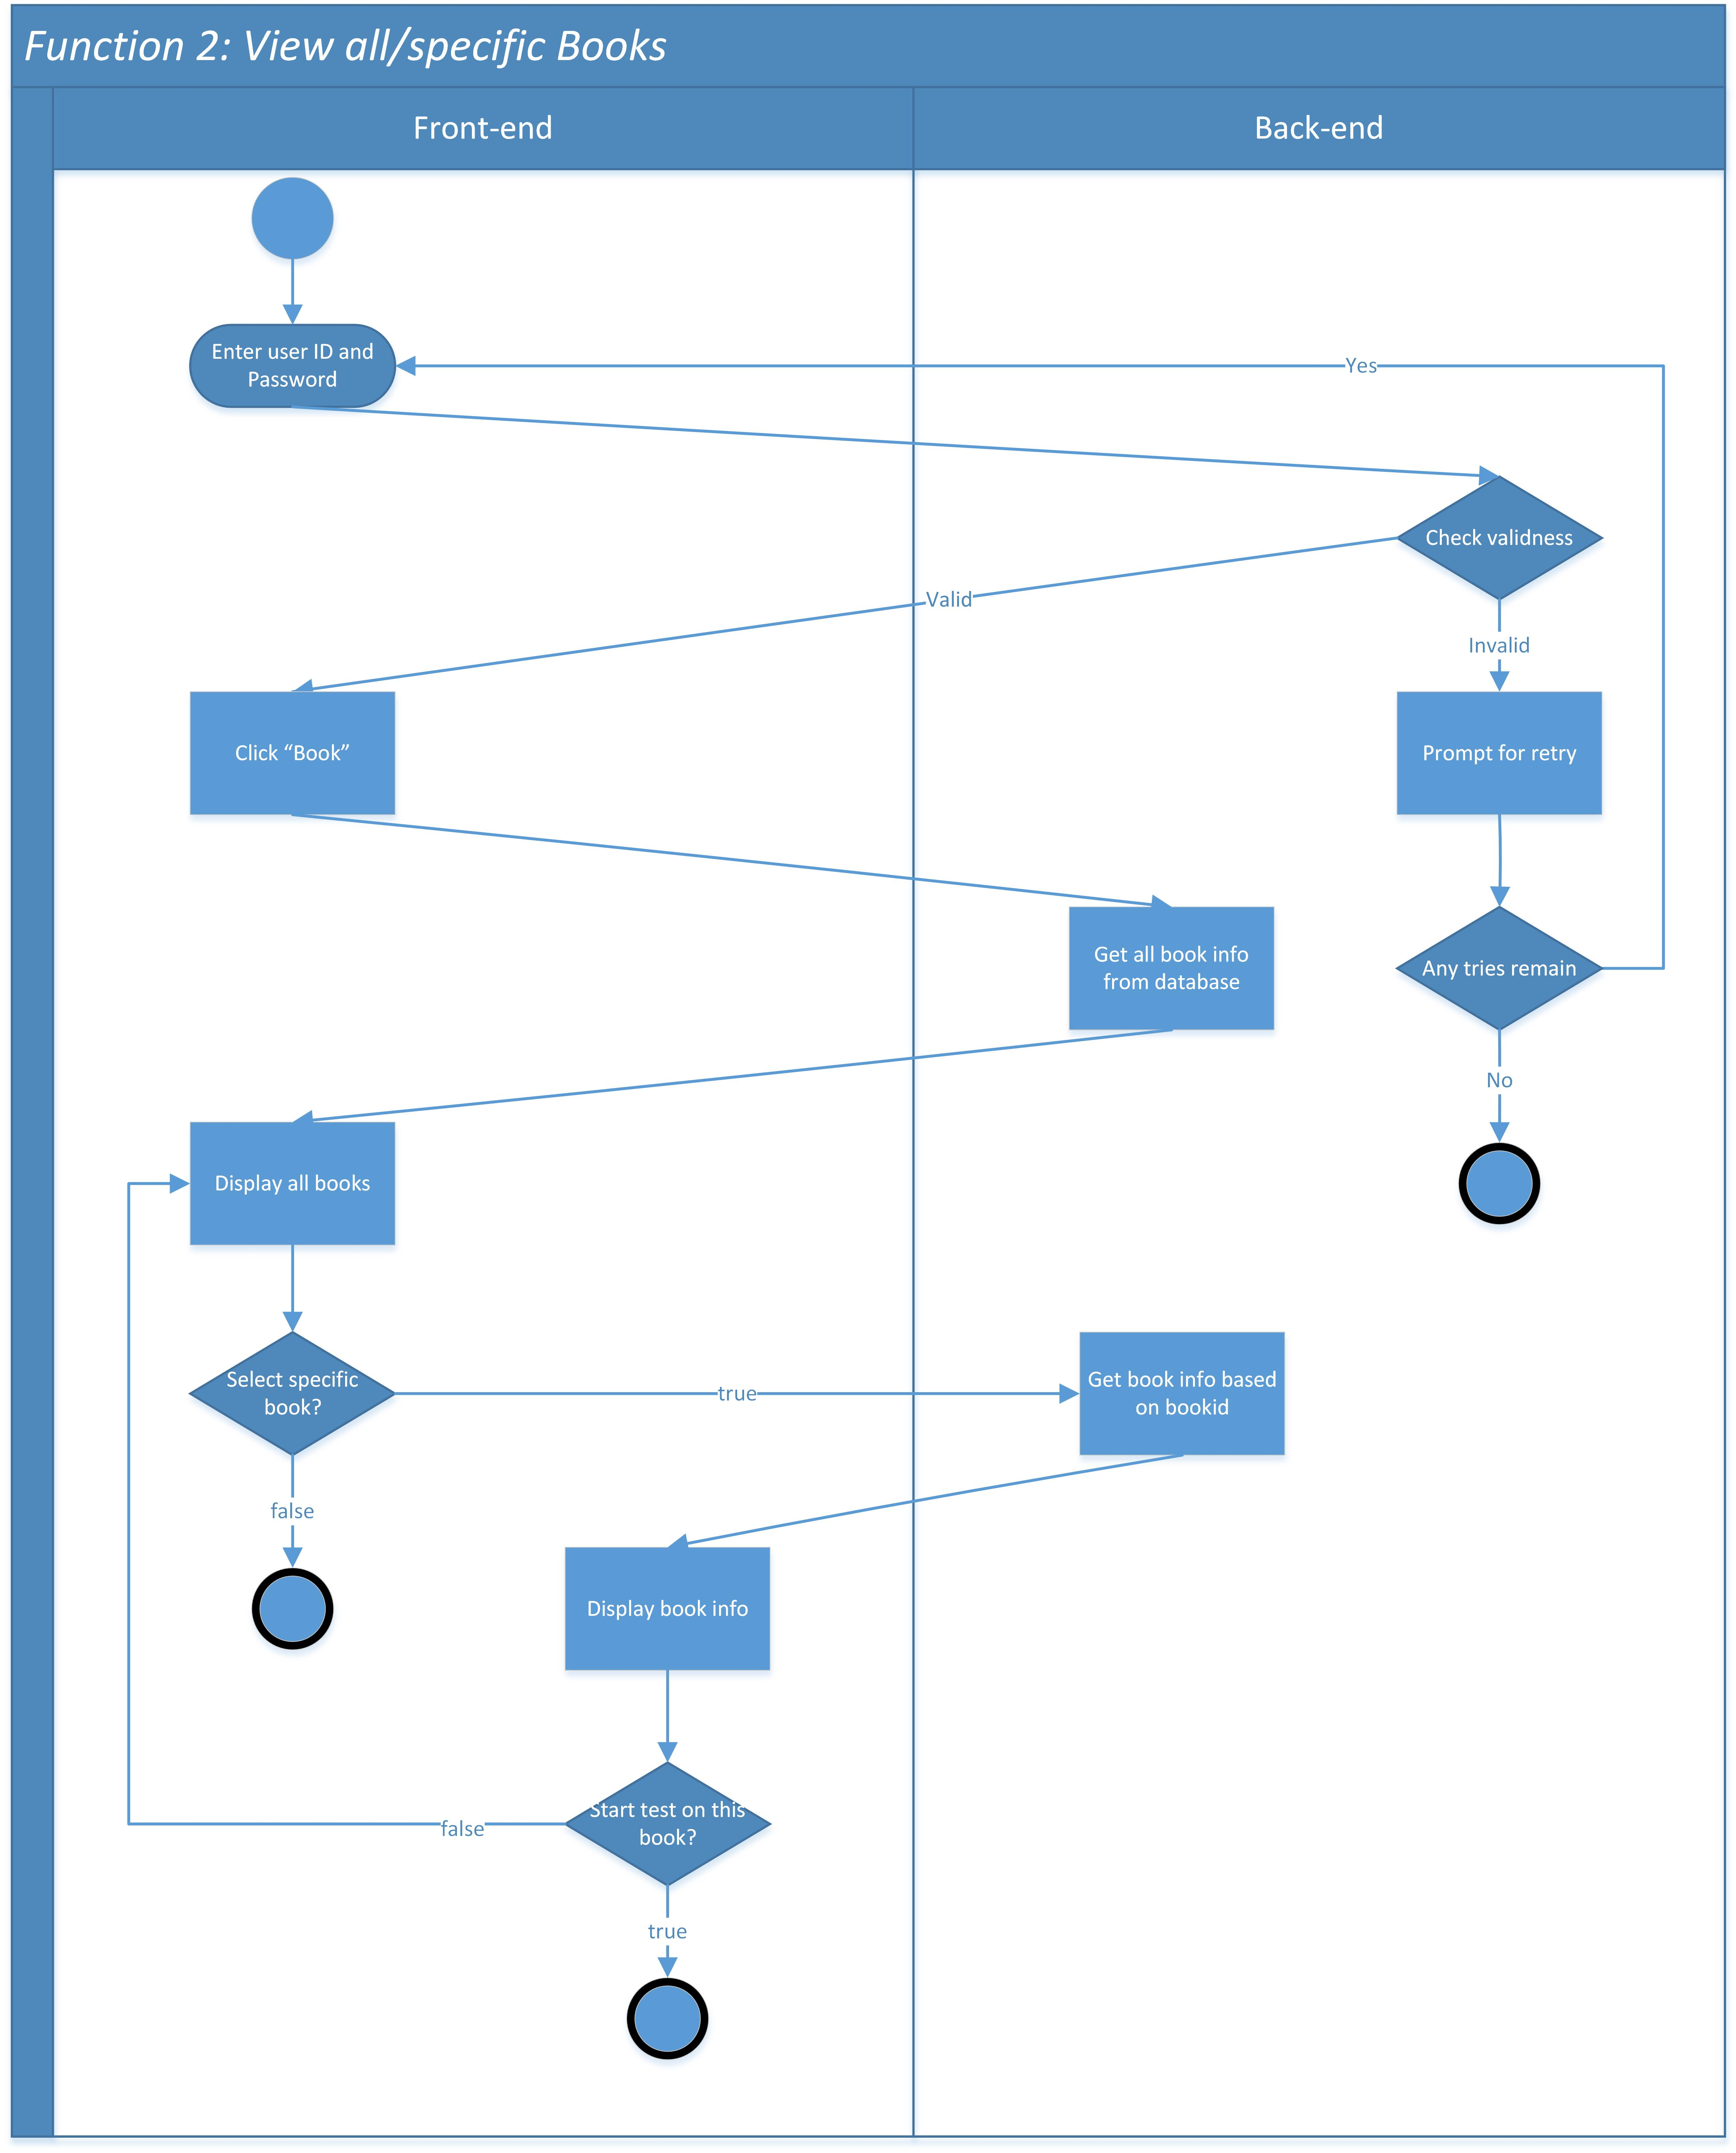
\includegraphics[width=0.9\columnwidth]{SwimLaneDiagram/Usecase_2.jpg}
    \caption{前后端交互:全部书籍信息预览}
    \label{fig:bookinfo}
\end{figure}
\newpage

\subsubsection{书籍信息测试}
\begin{figure}[H]
    \centering
    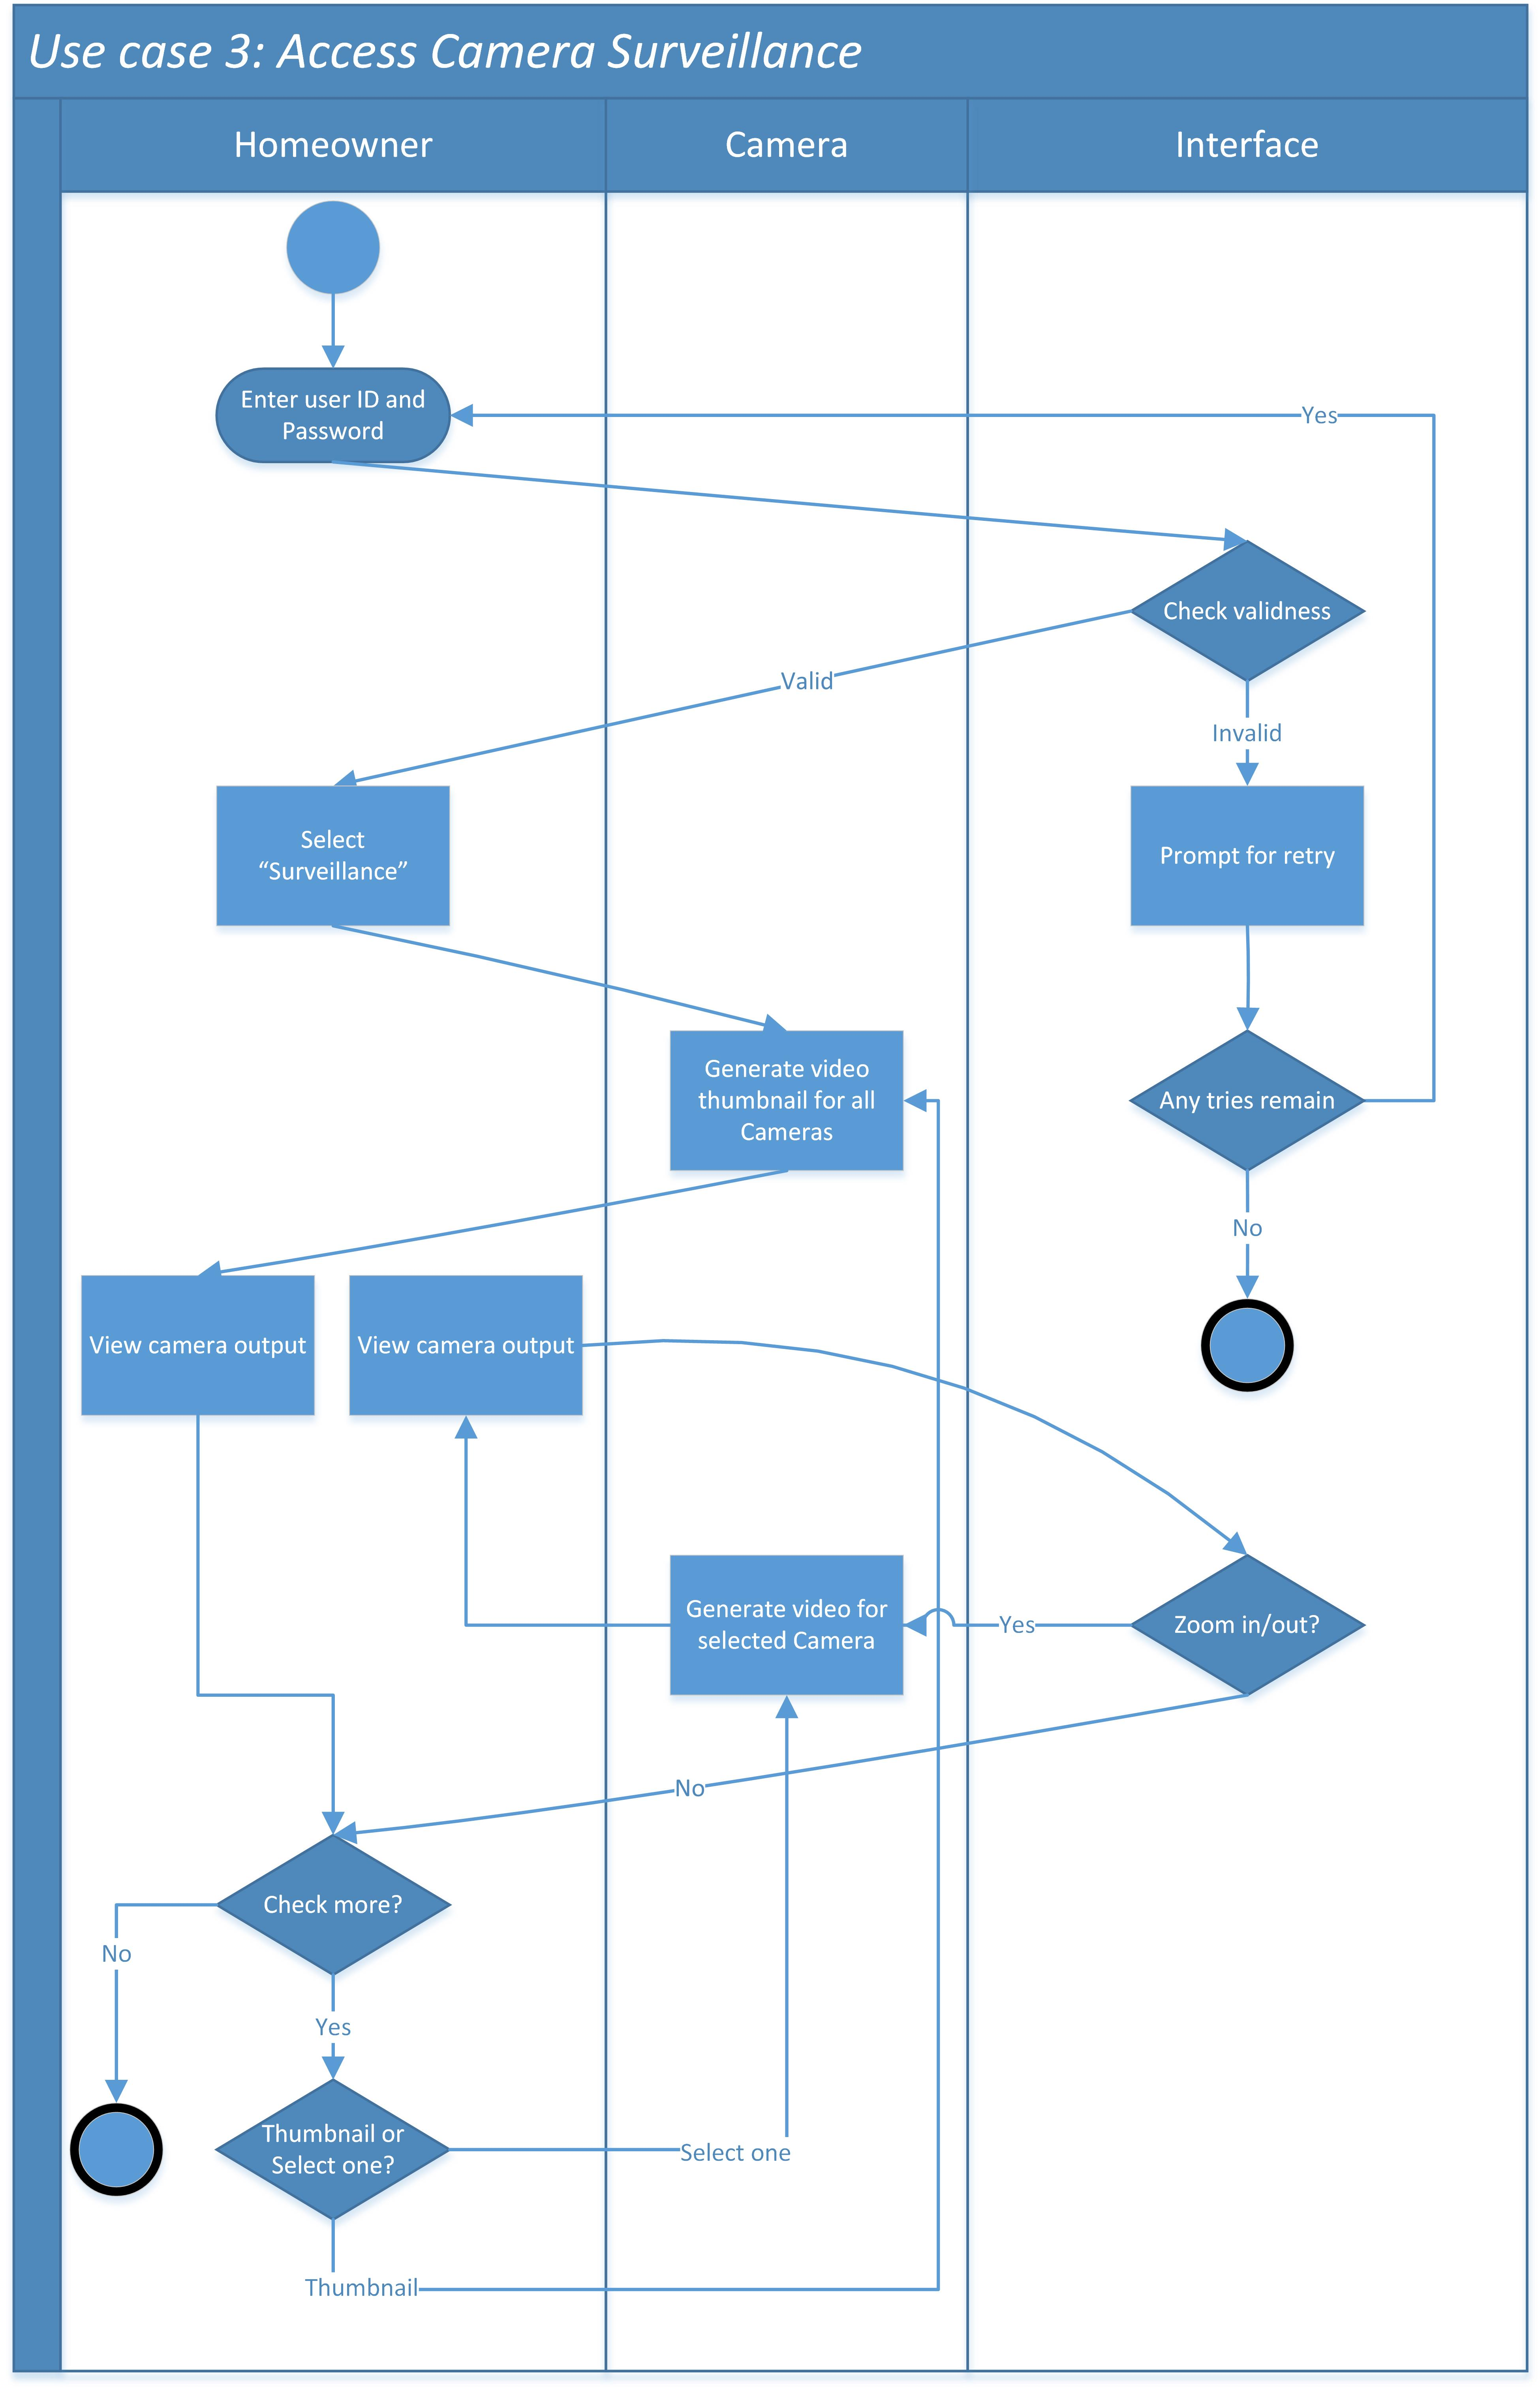
\includegraphics[width=0.8\columnwidth]{SwimLaneDiagram/Usecase_3.jpg}
    \caption{前后端交互:书籍信息测试}  
    \label{fig:test}
\end{figure}
\newpage

\subsubsection{测试结果分析以及可视化展示}
\begin{figure}[H]
    \centering
    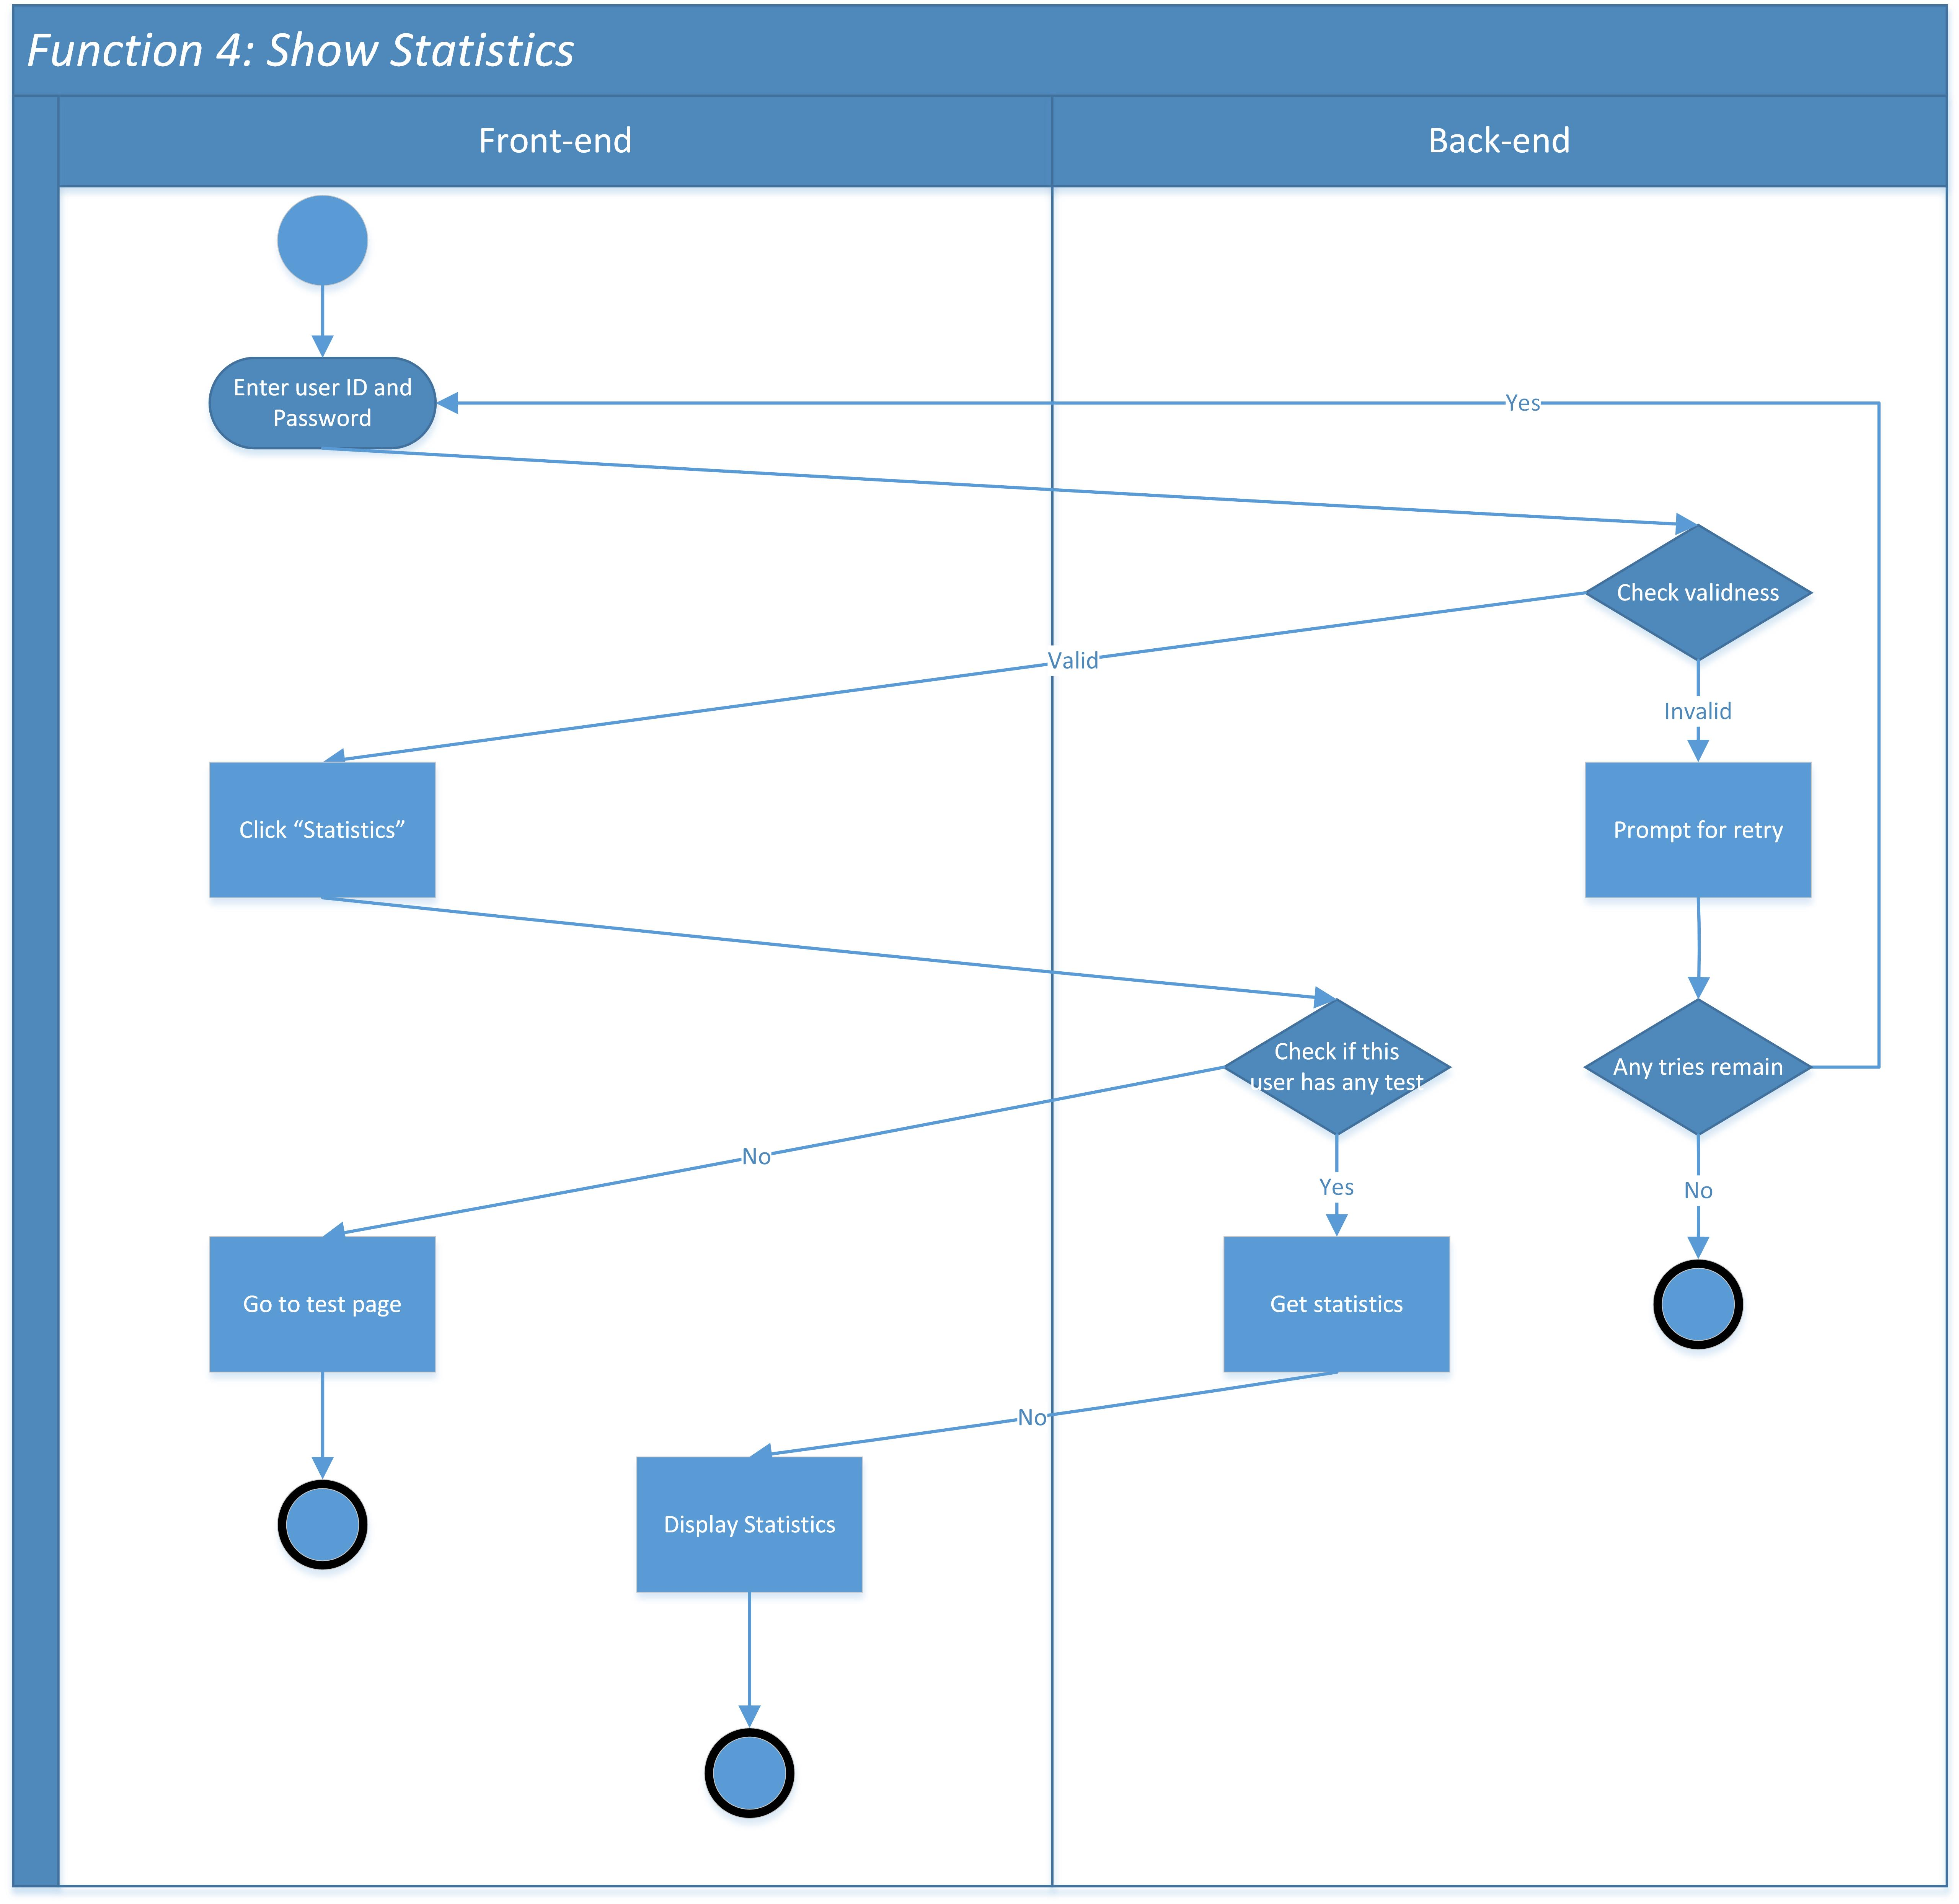
\includegraphics[width=1\columnwidth]{SwimLaneDiagram/Usecase_4.jpg}
    \caption{测试结果分析以及可视化展示}  
    \label{fig:statistics}
\end{figure}
\newpage

\section{结束语}

\subsection{总结}
\begin{enumerate}
    \item 在本次python课设项目中,是我们对于多人协作Coding的一次尝试,我们借助这次机会,去适应社区代码的提交,去了解和使用git这个强大的工具,他很好的让我们三人协同工作起来,并且在很多次爆出bug时拯救了我们。在我们的前期调研中,我们想把该项目做到较为满意的地步,而且对于程序员来说,合作也是一个在大学中需要主动去培养的技能,无论是在前期讨论分工,中期coding,后期报告、ppt制作答辩的哪个阶段,我们三人都学到了相关的知识和技能。
    \item 在本次python课设项目中,我们也是首次在类似课程设计的较大型项目中使用\LaTeX{}来进行报告撰写,也算是为了毕设和之后写论文做准备。在过程中也遇到了许多问题,比如:
          \begin{itemize}
              \item svg矢量图导入(Figure \ref{fig:backenduml})
              \item 将Author, Abstruct, Reference 加入到目录
              \item Reference 使用 BibTex
          \end{itemize}
    \item 在本次python课设项目中,我们也是首次去了解了Linux服务器。在中期的一次讨论中,我们遇到了前后端数据库不同步导致的问题,先是去尝试搭建局域网和云Sql服务器,但经过尝试后,遇到了很多问题,最后经过讨论觉得,如果可以全部部署到服务器一定会很炫酷。但过程是十分曲折的,虽然我们有一点点Linux的基础知识,但从零开始部署遇到了很多问题,而且在Linux下没有GUI界面,对于环境变量,软链接等的操作都更麻烦,我们也是debug了很久,才取得目前的成果。过程中也用到了计算机网络(端口控制,IP,域名)、操作系统(进程控制)等相关学科的知识。

\end{enumerate}
\subsection{不足与展望}

\begin{enumerate}
    \item 在前期准备中爬取了豆瓣Top200书籍的信息,但并未爬取完全,结果后期发现,豆瓣的Top200是根据评分数据一直在动态变化的。虽然后期通过豆瓣ID爬取出了全部的信息,但排名信息无法实时更新,后期会在此基础上继续改进。
    \item 在中期讨论中,想到把应用部署到服务器,便开始了对Linux服务器的探索,经过一周的尝试,最终有了我们自己的公网ip\href{http://47.116.46.195/}{\textbf{\emph{47.116.46.195}}},但由于备案时间需要半个月,我们的域名\href{http://www.castamerego.com/}{\textbf{\emph{http://www.castamerego.com/}}}未能在答辩时正式启用。
    \item 在过程中还存在很多问题,上面描述的只是部分,我们所遇到的全部问题可以点击\href{https://github.com/Casta-mere/Read-Book/tree/main/record/bugs}{\textbf{\emph{此处}}},在我们的Github仓库中查看。
\end{enumerate}

\phantomsection\addcontentsline{toc}{section}{Reference}\tolerance=500
\bibliography{references/references}

\end{document}
